\documentclass[
  aps,
  pra,
  reprint,
  superscriptaddress,
  nofootinbib,
  longbibliography
]{revtex4-2}

\usepackage{amsmath}
\usepackage{amssymb}
\usepackage{amsthm}
\usepackage{booktabs}
\usepackage{graphicx}
\usepackage{hyperref}
\hypersetup{
  hidelinks,
  pdftitle={Exact signed-sum spectral locus of a six-term three-qubit Pauli Hamiltonian},
  pdfauthor={Xiaojian Zeng}
}

\newtheorem{theorem}{Theorem}
\newtheorem{lemma}{Lemma}
\DeclareMathOperator{\Spec}{Spec}
\newcommand{\R}{\mathbb{R}}
\newcommand{\I}{\mathbb{I}}

\begin{document}

\title{Exact signed-sum spectral locus of a six-term three-qubit Pauli Hamiltonian}

\author{Xiaojian Zeng}
\email{xiaojianzeng@foxmail.com}
\affiliation{PBC School of Finance, Tsinghua University, Beijing 100190, China}

\date{15 September 2026}

\begin{abstract}
Free-fermion methods identify interacting-looking spin Hamiltonians whose many-body
energies are signed sums of single-particle energies.  We classify this spectral
property for the six-parameter three-qubit Hamiltonian
\(H=aZ_2+bY_1X_2+cX_1Y_2+dZ_1Y_3+eY_1X_3+fZ_3\), an example whose frustration
graph contains claws and even holes.  For arbitrary real couplings, its eight-level
spectrum is a multiset of the form
\(\{\pm\epsilon_1\pm\epsilon_2\pm\epsilon_3\}\), with three nonnegative
single-particle energies, if and only if
\[
 c d\,(a^2-f^2)(b^2-e^2)=0.
\]
Thus the complete real locus is the union of six hyperplanes: \(c=0\), \(d=0\),
\(a=\pm f\), and \(b=\pm e\).  The proof combines exact characteristic-polynomial
elimination with the chiral symmetry \(Y_1Y_2Y_3\).  The latter supplies a real
sufficiency argument and explicit nonnegative energies, including at zero and
degenerate strata.  This is a spectral classification only: it does not assert a
uniform Pauli-algebra construction of canonical fermion operators on the six
branches.
\end{abstract}

\maketitle

\section{Introduction}

Mappings from quantum spin Hamiltonians to noninteracting fermions can expose exact
spectra even when the required fermion operators are nonlinear and nonlocal in the
original spins.  A useful organizing object is the \emph{frustration graph}: its
vertices are Pauli terms and its edges record anticommutation.  Graph conditions such
as line-graph structure and the absence of claws or even holes lead to generic
free-fermion constructions \cite{Elman2021,Chapman2023}.  Other constructions reach
special spin-chain families outside the elementary Jordan--Wigner setting
\cite{FendleyPozsgay2024,FukaiVonaPozsgay2025}, while twin-collapse methods enlarge the
class identifiable from graph reductions \cite{RuhElman2026}.

The distinction between a free-fermion \emph{spectrum} and a structural fermion
mapping matters.  Spectrally, one asks whether all many-body energies can be written as
signed sums of nonnegative one-particle energies.  Structurally, one additionally asks
for canonical annihilation operators whose commutators reconstruct the Hamiltonian.
The former is necessary for the latter but does not, by itself, provide a useful local
or Pauli-algebra construction.

Elman, Chapman, and Flammia introduced the concrete Hamiltonian studied below and
observed numerically that its all-equal-coupling spectrum is free, although generic
couplings are not \cite{Elman2021}.  Its full six-term frustration graph has both claws
and even holes, so the generic graph criterion in that work does not settle its
fine-tuned coupling locus.  We determine the exact real \emph{spectral} locus.  The
answer replaces the single all-equal line by six complete hyperplanes and gives one
factorized polynomial obstruction everywhere else.

\section{Model and spectral question}
\label{sec:model}

On \((\mathbb{C}^{2})^{\otimes3}\), let \(X,Y,Z\) denote the standard Pauli matrices
and let a subscript specify the tensor factor.  We consider
\begin{equation}
 H=aZ_2+bY_1X_2+cX_1Y_2+dZ_1Y_3+eY_1X_3+fZ_3,
 \label{eq:H}
\end{equation}
with \((a,b,c,d,e,f)\in\R^6\).  The Pauli matrices are dimensionless, while all six
couplings have one common energy unit.  Equation~\eqref{eq:H} is a closed Hermitian
\(8\times8\) model; no thermodynamic, continuum, boundary, or perturbative limit is
taken.

For \(\boldsymbol\epsilon=(\epsilon_1,\epsilon_2,\epsilon_3)\in\R_{\geq0}^3\), define
the multiset
\begin{equation}
 \begin{aligned}
 \Sigma(\boldsymbol\epsilon)=\bigl\{&s_1\epsilon_1+s_2\epsilon_2+s_3\epsilon_3:\\
 &(s_1,s_2,s_3)\in\{-1,+1\}^3\bigr\}_{\rm mult}.
 \end{aligned}
 \label{eq:signedset}
\end{equation}
Zero \(\epsilon_j\) are permitted.  We seek all couplings for which
\(\Spec_{\rm mult}H=\Sigma(\boldsymbol\epsilon)\).  Although a general definition may
allow a common spectral shift, every term in Eq.~\eqref{eq:H} is traceless, so that
shift is necessarily zero.

The six Pauli words in the order \((a,b,c,d,e,f)\) are
\begin{equation}
 IZI,\quad YXI,\quad XYI,\quad ZIY,\quad YIX,\quad IIZ.
 \label{eq:words}
\end{equation}
The Pauli word
\begin{equation}
 \Gamma=Y_1Y_2Y_3
 \label{eq:gamma}
\end{equation}
satisfies \(\Gamma^2=\I\) and anticommutes with all six words in
Eq.~\eqref{eq:words}.  Hence \(\{\Gamma,H\}=0\), and Hermiticity gives
\begin{equation}
 \Spec_{\rm mult}H=\{\pm\lambda_1,\pm\lambda_2,
 \pm\lambda_3,\pm\lambda_4\}_{\rm mult}
 \label{eq:paired}
\end{equation}
for ordered magnitudes \(0\leq\lambda_1\leq\lambda_2\leq\lambda_3\leq\lambda_4\).

\section{Universal signed-sum polynomial}
\label{sec:universal}

Put \(t_j=\epsilon_j^2\), and let
\begin{equation}
 S_1=\sum_jt_j,\qquad
 S_2=\sum_{j<k}t_jt_k,\qquad
 S_3=t_1t_2t_3.
 \label{eq:Sdefs}
\end{equation}
Directly multiplying the eight factors associated with
Eq.~\eqref{eq:signedset} gives
\begin{align}
 \chi_{\rm ss}(E)
 ={}&E^8-4S_1E^6+(6S_1^2-8S_2)E^4 \notag\\
 &-4(S_1^3-4S_1S_2+16S_3)E^2
 +(S_1^2-4S_2)^2.
 \label{eq:universalpoly}
\end{align}
This identity is purely algebraic and does not yet guarantee that values inferred from
another polynomial are elementary symmetric functions of three nonnegative real
numbers.  That real-admissibility issue is handled in Sec.~\ref{sec:sufficiency}.

\section{Exact coupling locus}
\label{sec:locus}

Multiplication in the three-qubit Pauli group, followed by Newton identities for the
traces of \(H^k\), gives the first three even coefficients of \(\chi_H(E)\) in exactly
the form of Eq.~\eqref{eq:universalpoly}, with
\begin{align}
 S_1={}&a^2+b^2+c^2+d^2+e^2+f^2,
 \label{eq:S1}\\
 S_2={}&a^2d^2+a^2e^2+a^2f^2+b^2c^2+b^2e^2+b^2f^2
 \notag\\
 &{}+c^2f^2+d^2e^2,
 \label{eq:S2}\\
 S_3={}&a^2d^2e^2+b^2c^2f^2.
 \label{eq:S3}
\end{align}
The constant coefficient is
\begin{align}
 q_0={}&(S_1^2-4S_2)^2 \notag\\
 &{}-64c^2d^2(a-f)(a+f)(b-e)(b+e).
 \label{eq:q0}
\end{align}
Equations~\eqref{eq:S1}--\eqref{eq:q0} can also be verified by a direct exact
\(8\times8\) determinant.  No coupling or energy gap is divided out.

\begin{theorem}
\label{thm:locus}
For the Hamiltonian in Eq.~\eqref{eq:H}, there exist
\(\epsilon_1,\epsilon_2,\epsilon_3\geq0\) such that
\(\Spec_{\rm mult}H=\Sigma(\boldsymbol\epsilon)\) if and only if
\begin{equation}
 c d\,(a^2-f^2)(b^2-e^2)=0.
 \label{eq:locus}
\end{equation}
Equivalently, the complete real coupling locus is
\begin{equation}
 \begin{aligned}
 &\{c=0\}\cup\{d=0\}\cup\{a=f\}\cup\{a=-f\}\\
 &\hspace{3.7em}\cup\{b=e\}\cup\{b=-e\}.
 \end{aligned}
 \label{eq:union}
\end{equation}
No additional inequalities are required.
\end{theorem}

\begin{proof}[Necessity]
If the spectrum is a signed-sum multiset, its characteristic polynomial has the
constant coefficient in Eq.~\eqref{eq:universalpoly}.  Subtracting it from
Eq.~\eqref{eq:q0} yields the exact obstruction
\begin{equation}
 -64c^2d^2(a-f)(a+f)(b-e)(b+e),
 \label{eq:obstruction}
\end{equation}
which must vanish.  Over the real numbers this is equivalent to
Eq.~\eqref{eq:locus}.
\end{proof}

Figure~\ref{fig:slices} shows two coordinate slices of the four matched-coupling
components.  The remaining two components, \(c=0\) and \(d=0\), are coordinate
hyperplanes independent of the displayed pairs.

\begin{figure*}[t]
 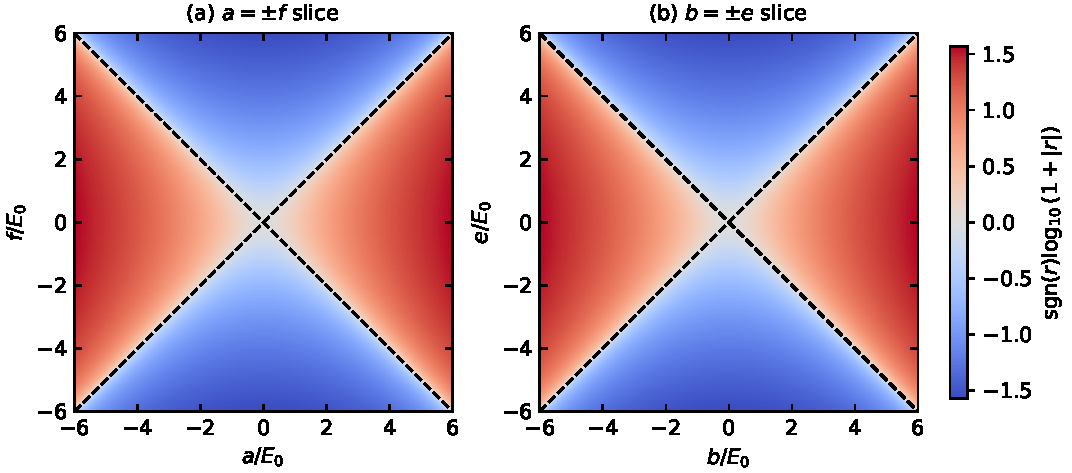
\includegraphics[width=0.91\textwidth]{figures/locus-slices.pdf}
 \caption{Two exact coordinate slices of the factorized obstruction in
 Eq.~\eqref{eq:obstruction}.  In (a), \((b,c,d,e)=(2,3,4,5)E_0\), so none of the
 omitted factors vanishes and the zero set is precisely \(a=\pm f\).  In (b),
 \((a,c,d,f)=(1,3,4,6)E_0\), and the zero set is \(b=\pm e\).  Color shows the
 signed monotone transform
 \(\operatorname{sgn}(r)\log_{10}(1+|r|)\), with
 \(r=(a^2-f^2)/E_0^2\) or \(r=(b^2-e^2)/E_0^2\); black dashed lines are the exact
 zero factors.  The plot is illustrative only; the classification follows from the
 exact factorization.}
 \label{fig:slices}
\end{figure*}

\section{Real sufficiency and explicit energies}
\label{sec:sufficiency}

It remains to show that a vanishing obstruction cannot hide complex or negative
solutions for the inferred \(t_j\).  The chiral pairing in Eq.~\eqref{eq:paired}
provides a direct proof.

\begin{proof}[Sufficiency]

Let \(y_i=\lambda_i^2\),
\begin{equation}
 U_1=\sum_{i=1}^4y_i,\qquad
 U_2=\sum_{1\leq i<j\leq4}y_iy_j,
 \qquad Q=4U_2-U_1^2.
 \label{eq:Udefs}
\end{equation}
Comparing the \(E^6\) and \(E^4\) coefficients of \(\chi_H\) with
Eq.~\eqref{eq:universalpoly} gives
\begin{equation}
 S_1=\frac{U_1}{4},\qquad S_1^2-4S_2=\frac{Q}{8}.
 \label{eq:SQ}
\end{equation}
On the locus \eqref{eq:locus}, equality of the constant coefficients becomes
\begin{equation}
 64(\lambda_1\lambda_2\lambda_3\lambda_4)^2-Q^2=0.
 \label{eq:lambdaobstruction}
\end{equation}
Its left-hand side factors exactly as
\begin{equation}
 -\!\!\prod_{\sigma_2,\sigma_3,\sigma_4\in\{-1,+1\}}
 (\lambda_1+\sigma_2\lambda_2+\sigma_3\lambda_3+
 \sigma_4\lambda_4).
 \label{eq:linearproduct}
\end{equation}

With the stated ordering of the four magnitudes, a zero factor is equivalent to one of
the two relations
\begin{align}
 \lambda_4&=\lambda_1+\lambda_2+\lambda_3,
 \label{eq:caseA}\\
 \lambda_4+\lambda_1&=\lambda_2+\lambda_3.
 \label{eq:caseB}
\end{align}
Indeed, after fixing the overall sign so that \(\lambda_4\) is positive, the remaining
nontrivial partitions besides Eqs.~\eqref{eq:caseA} and \eqref{eq:caseB} contain either
\((\lambda_4-\lambda_3)+(\lambda_2-\lambda_1)\) or
\((\lambda_4-\lambda_2)+(\lambda_3-\lambda_1)\).  Equality forces paired coincidences
and hence a subcase of Eq.~\eqref{eq:caseB}.  The partitions with three or four positive
terms can vanish only in the corresponding zero subcases.

For Eq.~\eqref{eq:caseA}, choose
\begin{equation}
 (\epsilon_1,\epsilon_2,\epsilon_3)
 =\frac12(\lambda_2+\lambda_3,\lambda_1+\lambda_3,
 \lambda_1+\lambda_2).
 \label{eq:epsA}
\end{equation}
The four magnitudes obtained from the signed sums are
\(\lambda_4,\lambda_3,\lambda_2,\lambda_1\).  For Eq.~\eqref{eq:caseB}, choose
\begin{equation}
 (\epsilon_1,\epsilon_2,\epsilon_3)
 =\frac12(\lambda_4+\lambda_1,\lambda_4-\lambda_2,
 \lambda_4-\lambda_3).
 \label{eq:epsB}
\end{equation}
Ordering makes every entry nonnegative, and the four signed sums modulo overall sign
again have magnitudes \(\lambda_4,\lambda_3,\lambda_2,\lambda_1\).  Equations
\eqref{eq:epsA} and \eqref{eq:epsB} remain valid when magnitudes vanish or coincide.
They prove sufficiency in Theorem~\ref{thm:locus} without assuming positivity of roots
of an inferred cubic.
\end{proof}

\section{Boundary strata and scope}
\label{sec:boundaries}

Because the proof never cancels a coupling, Eq.~\eqref{eq:union} includes the origin,
all intersections, and all coordinate-zero strata.  On the locus, a zero
single-particle energy occurs exactly when \(S_3=0\), or equivalently
\begin{equation}
 ade=0\quad\text{and}\quad bcf=0.
 \label{eq:zeromode}
\end{equation}
At least two single-particle energies vanish exactly when \(S_2=0\); all three vanish
only at the origin.  Repeated squared single-particle energies are retained on the
discriminant
\begin{equation}
 \Delta_t=S_1^2S_2^2-4S_2^3-4S_1^3S_3-27S_3^2
 +18S_1S_2S_3=0,
 \label{eq:discriminant}
\end{equation}
and no part of that set is lost from the sufficiency argument.

The result should not be read as a claim of scalable free-fermion simulation.  At the
unrestricted finite-dimensional level, any spectrum of the form
Eq.~\eqref{eq:signedset} permits a canonical fermion triple after choosing and labeling
an eigenbasis.  Such a construction is tautological and generally carries no locality
or efficient Pauli representation.  The nontrivial open structural question is to
construct coupling-dependent canonical modes in the Pauli algebra, with controlled
limits at degeneracies, especially on the four fine-tuned components \(a=\pm f\) and
\(b=\pm e\).  Theorem~\ref{thm:locus} establishes only the exact multiset condition
required before such a construction can exist.

\section{Published limit and reproducibility}
\label{sec:reproducibility}

For the published all-equal limit \(a=b=c=d=e=f=J\), anticommutation of the words in
Eq.~\eqref{eq:words} gives independent-set counts \((1,6,8,2)\).  At \(J=1\), the
weighted independence-polynomial rule of Ref.~\cite{Elman2021} gives squared
one-particle energies equal to the three positive roots of
\begin{equation}
 t^3-6t^2+8t-2=0.
 \label{eq:baselinecubic}
\end{equation}
Both the signed sums and the matrix in Eq.~\eqref{eq:H} then have characteristic
polynomial
\begin{equation}
 E^8-24E^6+152E^4-224E^2+16.
 \label{eq:baselinepoly}
\end{equation}
This reproduces the reported all-equal spectrum, while Theorem~\ref{thm:locus} shows
that the line lies in the intersection \(a=f\) and \(b=e\).

The accompanying source package contains two independent Hamiltonian reconstructions:
one uses Kronecker products of explicit Pauli matrices, and the other acts column by
column on computational-basis bits using
\(Y|q\rangle=i(-1)^q|1-q\rangle\).  They agree entrywise in exact symbolic arithmetic.
A third implementation multiplies elements of the Pauli group, computes
\(\operatorname{tr}H^k\) through \(k=8\), and applies Newton identities.  It reproduces
Eqs.~\eqref{eq:S1}--\eqref{eq:q0} without importing the matrix code.  Scripts also
verify Eqs.~\eqref{eq:linearproduct}--\eqref{eq:epsB} and regenerate
Fig.~\ref{fig:slices}.  The decisive equalities use exact integer and symbolic
arithmetic; floating-point diagonalizations are retained only as diagnostics.

\section{Conclusion}

The free-spectral locus of the six-term Hamiltonian \eqref{eq:H} is exactly the union
of the six hyperplanes in Eq.~\eqref{eq:union}.  The factorization
Eq.~\eqref{eq:obstruction} excludes every off-locus real coupling, while chiral
symmetry converts the same condition into a linear relation among four ordered
spectral magnitudes and thereby yields nonnegative one-particle energies.  The
classification is exact at all zero and degenerate intersections.  It sharpens a
single numerical fine-tuned observation into a complete finite-model coupling-space
statement, while leaving structural canonical-mode constructions as a separate
problem.

\begin{acknowledgments}
OpenAI Codex (model \texttt{gpt-5.6-sol}, accessed in September 2026) assisted with
primary-literature discovery, symbolic-derivation exploration, code generation,
independent computational checks, figure preparation, and manuscript drafting.  It
was directed to preserve the fixed Hamiltonian and exact real-coupling scope.  Its
outputs were tested through separately implemented Kronecker-product,
computational-bit, and Pauli-group/Newton calculations.  AI tools are not authors;
final scientific and textual verification and responsibility for any submitted
version belong to the author.
\end{acknowledgments}

\section*{Data and code availability}
No experimental data were used.  All equations needed for the central result appear in
the article.  Exact verification and figure-generation scripts, environment versions,
and regeneration instructions are included in the accompanying source package.

\bibliography{references}

\end{document}
